\documentclass{standalone}
%
\usepackage{tikz,xcolor}
\usetikzlibrary{shapes.geometric,arrows,positioning,fit,calc}
\tikzstyle{arrow} = [thick,->,>=stealth]

\begin{document}
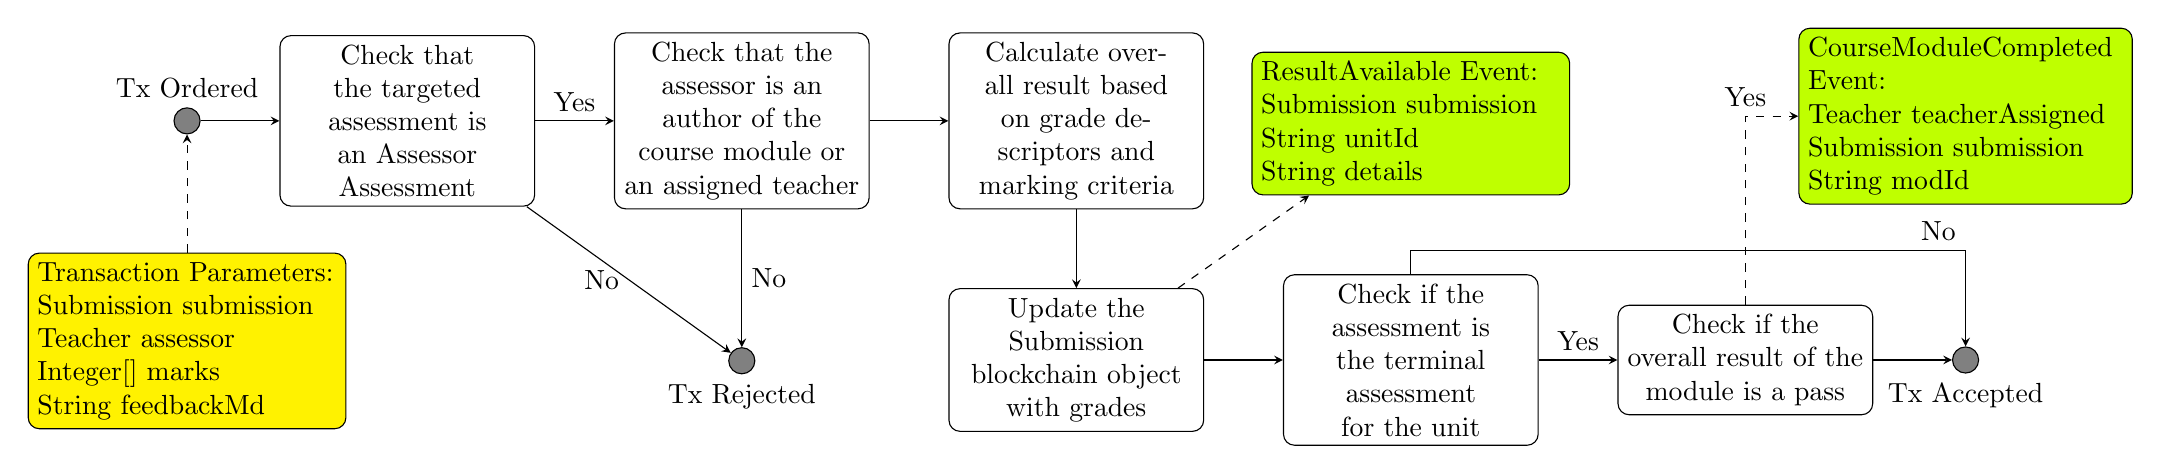
\begin{tikzpicture}[>=stealth,every node/.style={shape=rectangle,draw,rounded corners},]
    % create the nodes
    \node (start)[shape=circle, fill=gray, label=above:Tx Ordered] {};
    \node (param)[below = 1.5cm of start, text width=3.8cm, fill=yellow]{Transaction Parameters:\\Submission submission\\Teacher assessor\\Integer[] marks\\String feedbackMd};  
    \node (c1) [right = of start, text width=3cm, align=center]{Check that the targeted assessment is an Assessor Assessment};
    \node (c2) [right = of c1, text width=3cm, align=center]{Check that the assessor is an author of the course module or an assigned teacher};
    \node (stop1)[below = 1.75cm of c2, shape=circle, fill=gray, label=below:Tx Rejected] {};        
    \node (c3) [right = of c2, text width=3cm, align=center]{Calculate overall result based on grade descriptors and marking criteria};    
    \node (c4) [below = of c3, text width=3cm, align=center]{Update the Submission blockchain object with grades};    
    \node (c5) [right = of c4, text width=3cm, align=center]{Check if the assessment is the terminal assessment for the unit};
    \node (c6) [right = of c5, text width=3cm, align=center]{Check if the overall result of the module is a pass};
    \node (event1)[above =of c5, text width=3.8cm, fill=lime]{ResultAvailable Event:\\ Submission submission\\String unitId \\ String details };
    \node (stop2)[right = of c6, shape=circle, fill=gray, label=below:Tx Accepted] {};    
    \node (event2)[above = 1.8cm of stop2, text width=4cm, fill=lime]{CourseModuleCompleted Event:\\ Teacher teacherAssigned\\Submission submission \\ String modId };    

    % connect the nodes
    \draw[->, dashed] (param) to (start);    
    \draw[->] (start) to (c1);
    \draw[->] (c1) -- node[draw=none, anchor=south] {Yes} (c2);  
    \draw[->] (c1) -- node[draw=none, anchor=east] {No} (stop1);    
    \draw[->] (c2) -- node[draw=none, anchor=west] {No} (stop1);         
    \draw[->] (c2) to (c3);
    \draw[->] (c3) to (c4);
    \draw[->] (c4) to (c5);
    \draw[->] (c5) -- node[draw=none, anchor=south] {Yes} (c6);  
    \draw[->] (c5.north) --($(c5.north)+(0,0.3)$)-| node[draw=none, anchor=south east] {No} (stop2.north);          
    \draw[->] (c6) to (stop2);
    \draw[->, dashed] (c4) to (event1);        
    \draw[->, dashed] (c6.north) |- node[draw=none, anchor=south] {Yes} (event2.west);        

\end{tikzpicture}
\end{document}
